% *********************************************************************
% © 2021–2024 Jeremy Sylvestre
%
% Permission is granted to copy, distribute and/or modify this document
% under the terms of the GNU Free Documentation License, Version 1.3 or
% any later version published by the Free Software Foundation; with no
% Invariant Sections, no Front-Cover Texts, and no Back-Cover Texts. A
% copy of the license is included in the appendix entitled “GNU Free
% Documentation License” that appears in the output document of this
% PreTeXt source code. All trademarks™ are the registered® marks of
% their respective owners.
%
% *********************************************************************

\newcommand*{\xmin}{-0.075}
\newcommand*{\xmax}{1.1}
\newcommand*{\ymin}{-0.25}
\newcommand*{\ymax}{2.5}

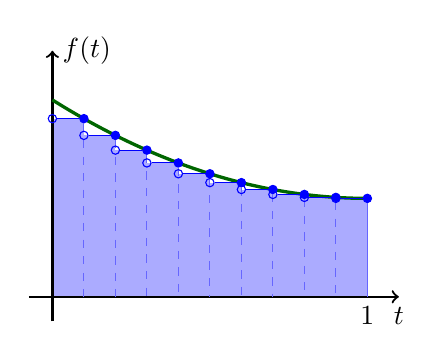
\begin{tikzpicture}
[
	closedpt/.style={circle,draw,fill,inner sep=0pt,minimum size=3pt},
	openpt/.style={circle,draw,inner sep=0pt,minimum size=3pt},
	xscale=4,yscale=1.25
]

	% rectangle fills
	\fill[blue, opacity=0.33] (0,1.81) rectangle (0.1,0);
	\fill[blue, opacity=0.33] (0.1,1.64) rectangle (0.2,0);
	\fill[blue, opacity=0.33] (0.2,1.49) rectangle (0.3,0);
	\fill[blue, opacity=0.33] (0.3,1.36) rectangle (0.4,0);
	\fill[blue, opacity=0.33] (0.4,1.25) rectangle (0.5,0);
	\fill[blue, opacity=0.33] (0.5,1.16) rectangle (0.6,0);
	\fill[blue, opacity=0.33] (0.6,1.09) rectangle (0.7,0);
	\fill[blue, opacity=0.33] (0.7,1.04) rectangle (0.8,0);
	\fill[blue, opacity=0.33] (0.8,1.01) rectangle (0.9,0);
	\fill[blue, opacity=0.33] (0.9,1) rectangle (1,0);

	% label horiz axis
	\node[below] at (1,0) {$1$};

	% axes
	\draw[->,thick] (\xmin,0) -- (\xmax,0) node[below] {$t$};
	\draw[->,thick] (0,\ymin) -- (0,\ymax) node[right] {$f(t)$};

	% continuous graph
	\draw[green!40!black,very thick,domain=0:1,smooth] plot (\x,{\x^2 - 2 * \x + 2});

	% levels and dividers
	\node[blue,openpt] at (0,1.81) (start) {};
	\node[blue,closedpt] at (0.1,1.81) (stop) {};
	\draw[blue,thin] (start.east) -- (stop.west);
	\draw[blue!60!white,dashed] (stop.south) -- (0.1,0);
	%
	\node[blue,openpt] at (0.1,1.64) (start) {};
	\node[blue,closedpt] at (0.2,1.64) (stop) {};
	\draw[blue,thin] (start.east) -- (stop.west);
	\draw[blue!60!white,dashed] (stop.south) -- (0.2,0);
	%
	\node[blue,openpt] at (0.2,1.49) (start) {};
	\node[blue,closedpt] at (0.3,1.49) (stop) {};
	\draw[blue,thin] (start.east) -- (stop.west);
	\draw[blue!60!white,dashed] (stop.south) -- (0.3,0);
	%
	\node[blue,openpt] at (0.3,1.36) (start) {};
	\node[blue,closedpt] at (0.4,1.36) (stop) {};
	\draw[blue,thin] (start.east) -- (stop.west);
	\draw[blue!60!white,dashed] (stop.south) -- (0.4,0);
	%
	\node[blue,openpt] at (0.4,1.25) (start) {};
	\node[blue,closedpt] at (0.5,1.25) (stop) {};
	\draw[blue,thin] (start.east) -- (stop.west);
	\draw[blue!60!white,dashed] (stop.south) -- (0.5,0);
	%
	\node[blue,openpt] at (0.5,1.16) (start) {};
	\node[blue,closedpt] at (0.6,1.16) (stop) {};
	\draw[blue,thin] (start.east) -- (stop.west);
	\draw[blue!60!white,dashed] (stop.south) -- (0.6,0);
	%
	\node[blue,openpt] at (0.6,1.09) (start) {};
	\node[blue,closedpt] at (0.7,1.09) (stop) {};
	\draw[blue,thin] (start.east) -- (stop.west);
	\draw[blue!60!white,dashed] (stop.south) -- (0.7,0);
	%
	\node[blue,openpt] at (0.7,1.04) (start) {};
	\node[blue,closedpt] at (0.8,1.04) (stop) {};
	\draw[blue,thin] (start.east) -- (stop.west);
	\draw[blue!60!white,dashed] (stop.south) -- (0.8,0);
	%
	\node[blue,openpt] at (0.8,1.01) (start) {};
	\node[blue,closedpt] at (0.9,1.01) (stop) {};
	\draw[blue,thin] (start.east) -- (stop.west);
	\draw[blue!60!white,dashed] (stop.south) -- (0.9,0);
	%
	\node[blue,openpt] at (0.9,1) (start) {};
	\node[blue,closedpt] at (1,1) (stop) {};
	\draw[blue,thin] (start.east) -- (stop.west);
	\draw[blue!60!white] (stop.south) -- (1,0);
	%

\end{tikzpicture}
